\subsection{Escenario de referencia}

Para aplicar NFS a un datacenter puede considerarse un escenario con varios servidores fisicos de computo conectados a una red Ethernet de alta velocidad y a una cabina o servidor de almacenamiento que exporta directorios mediante NFS. Los nodos ejecutan aplicaciones, maquinas virtuales, contenedores o procesos distribuidos que necesitan acceder a un conjunto comun de archivos.

En este escenario, NFS no es un recurso aislado sino un servicio de red critico. Cada lectura o escritura remota consume ancho de banda, agrega latencia y depende de switches, interfaces, rutas, firewalls y del servidor de almacenamiento. Por eso, la arquitectura de red es tan importante como la configuracion del propio servicio NFS.

\subsection{VLAN dedicada para tráfico NFS}

Una practica comun en datacenters es separar el trafico de almacenamiento del trafico de produccion y del trafico de gestion. Para ello se puede definir una VLAN dedicada, por ejemplo \textbf{VLAN 30}, utilizada exclusivamente para NFS. Los servidores tendrian al menos una interfaz o subinterfaz dentro de esa VLAN, y el servidor NAS/NFS tendria interfaces de almacenamiento en la misma red.

La VLAN dedicada no reemplaza autenticacion, cifrado ni permisos. Su funcion principal es reducir contencion, limitar exposicion lateral y facilitar la operacion de red. Si NFS comparte enlaces y colas con trafico de usuarios, backups o administracion, una carga intensa de E/S puede afectar servicios no relacionados. Separar el plano de almacenamiento permite aplicar politicas especificas de QoS, monitoreo y filtrado.

\begin{figure}[H]
    \centering
    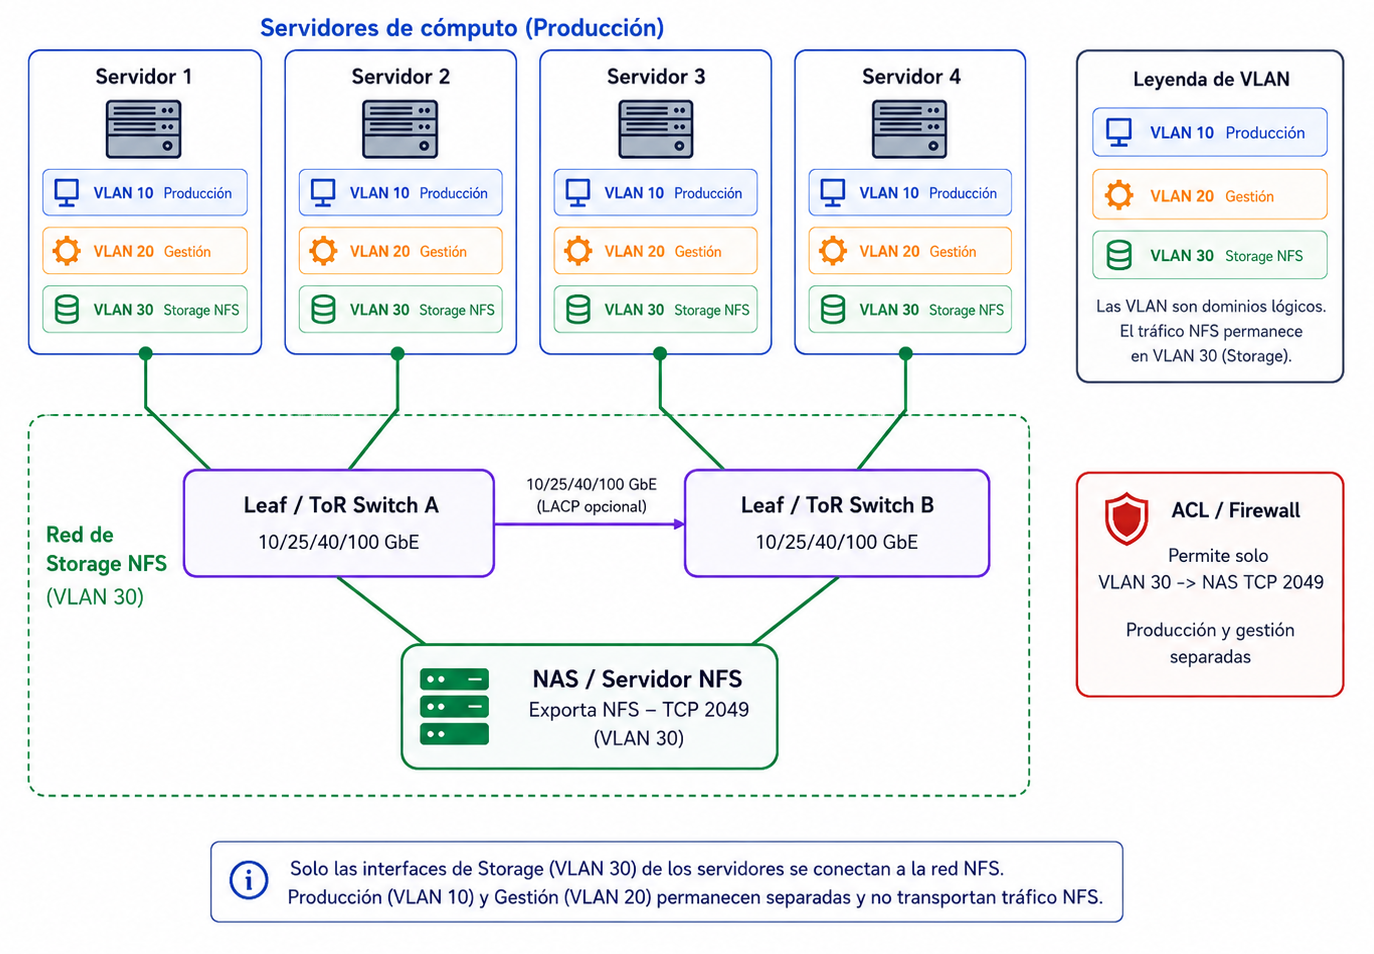
\includegraphics[width=0.95\textwidth]{img/nfs_03.png}
    \caption{VLAN NFS en datacenter}
    \label{fig:nfs_datacenter_vlan}
\end{figure}

\subsection{Diseño físico y redundancia de red}

En produccion, los servidores no deberian depender de una unica interfaz ni de un unico switch. Una configuracion habitual consiste en conectar cada host a dos switches ToR o leaf distintos. Las interfaces pueden operar mediante bonding, teaming o LACP, segun el sistema operativo y el diseño de red. El objetivo no es solo sumar ancho de banda, sino eliminar puntos unicos de falla.

El ancho de banda necesario depende de la carga. Para usos moderados, 10 GbE puede ser suficiente. En virtualizacion, procesamiento de archivos grandes o muchos hosts accediendo simultaneamente, 25 GbE o superior ofrece mas margen. De todos modos, aumentar la velocidad fisica no garantiza por si solo mayor rendimiento si el cuello de botella esta en el servidor NFS, la CPU, las conexiones TCP o el backend de discos.

\subsection{Diseño recomendado para el escenario propuesto}

Una implementacion razonable para el escenario analizado seria usar servidores con interfaces redundantes, una VLAN de produccion para las aplicaciones, una VLAN de gestion para administracion y una VLAN de almacenamiento para NFS. El servidor NFS o cabina NAS exportaria recursos accesibles solo desde la subred de computo.

La version recomendada seria NFSv4.1 como base, por su equilibrio entre interoperabilidad, simplificacion de puertos y locking integrado. Para datos sensibles puede evaluarse Kerberos con \texttt{sec=krb5i} o \texttt{sec=krb5p}; para datos internos menos criticos podria utilizarse \texttt{sec=sys}, siempre que exista aislamiento de red, control estricto por subred y permisos coherentes.
